%%%%%%%%%%%%%%%%%%%%%%%%%%%%%%%%%%%%%%%%%
% University/School Laboratory Report
% LaTeX Template
% Version 3.1 (25/3/14)
%
% This template has been downloaded from:
% http://www.LaTeXTemplates.com
%
% Original author:
% Linux and Unix Users Group at Virginia Tech Wiki 
% (https://vtluug.org/wiki/Example_LaTeX_chem_lab_report)
%
% License:
% CC BY-NC-SA 3.0 (http://creativecommons.org/licenses/by-nc-sa/3.0/)
%
%%%%%%%%%%%%%%%%%%%%%%%%%%%%%%%%%%%%%%%%%

%----------------------------------------------------------------------------------------
%	PACKAGES AND DOCUMENT CONFIGURATIONS
%----------------------------------------------------------------------------------------

\documentclass{article}

\usepackage[utf8]{inputenc}
\usepackage{graphicx} % Required for the inclusion of images
%\usepackage{natbib} % Required to change bibliography style to APA
\usepackage{amsmath} % Required for some math elements 
\usepackage{glossaries}
\usepackage[toc,page]{appendix}
\usepackage[autostyle=true]{csquotes}
\usepackage{hyperref}
\usepackage{amssymb}
\usepackage{caption} 
\usepackage{hhline}
\usepackage{float}
\usepackage{listings}

\setlength\parindent{0pt} % Removes all indentation from paragraphs

%\usepackage{times} % Uncomment to use the Times New Roman font

%----------------------------------------------------------------------------------------
%	DOCUMENT INFORMATION
%----------------------------------------------------------------------------------------

\title{Pure by Nature:\\A Library for Agent-Based Simulation \& Modelling in Haskell} % Title

\author{Jonathan \textsc{Thaler}} % Author name

\date{\today} % Date for the report

\begin{document}

\maketitle % Insert the title, author and date

% If you wish to include an abstract, uncomment the lines below
\begin{abstract}
TODO: the title is not very well suited towards research: it just describes the implementation of a library which is just of a software-engineering problem and not a research topic.

Stability of emergent properties of ABM/S under different Simulation-Semantics.

The central research of this paper is
- establishing a terminology for speaking about Simulation-Semantics
- how do emergent properties behave under varying simulation semantics?
	-> for this we implemented same model in different languages: Java, Haskell and Scala & Actors with different Simulation-Semantics: Java & Haskell all Global, Scala & Actors Local only.
	-> Java: supports global data => suitable to implement global decisions: implementing global-time, sequential iteration with global decisions
	-> Haskell: has no global data => local decisions (has support for global data through STM/IO but then looses very power?) => implementing global-time, parallel iteration with local-decisions. 
		-> Haskell STM solution => implementing concurrent version using STM? but this is very complicated in its own right but utilizing STM it will be much more easier than in java
	-> Scala: mixed, can do both => implementing local time with random iteration and local decisions
- can we reason about emergent properties / dynamics of a simulation just by looking at the code/model or is it impossible?
	-> hypothesis: it all depends on the way we formulate our problem: we might be able to tell from the model-specification but code could become too complicated
		=> if we write code that looks same as the model-specification (using an EDSL) we could potentially be able to identify:
			-> positive & negative feedback-loops 
			-> other mechanisms of feedback/sources of emergent properties?
				-> what are sources of emergent properties?
					-> what are emergent properties anyway? can we deliver a very precise definition?

=> we see that using different update-strategies, different patterns emerge e.g. in Scala & Actors
=> STM solution is much slower than the par-version without yet using parallel-execution!

In this paper we look at the very simple social-simulation of \textit{Heroes \& Cowards} invented by \cite{wilensky_introduction_2015} to study new methods in Agent-Based Modelling and Simulation (ABM/S) and to highlight their potentials and limitations as opposed to object-oriented (OO) ones which are dominant in this field. We go into the opposite direction and ask how ABM/S can be done using the Actor-Model as defined by \cite{agha_actors:_1986} and pure functional programming in Haskell. Both are methods which have unfortunately not been considered very deeply in this field and requires to look at ABM/S from a different perspective which this paper tries to provide. The Actor-Model was a major influence in the development of Agents and has proven its use in Erlang for building industry-strength applications but the question whether it is well suited for ABM/S is still open to question. A functional direction offers a wealth of new powerful tools and methods where the most obvious benefits of using a pure functional approach is that it allows to reason about various properties of the program and implementation of an embedded domain-specific language (EDSL), where ideally the distinction between specification and implementation disappears. \\
Thus we implemented a new library in Haskell for ABM/S called \textit{PureAgents}, available on Hackage, making maximum use of the functional paradigm and utilizing the Actor-Model as the underlying paradigm for thinking, representing, modelling and implementing Agents. We compare the implementation of \textit{Heroes \& Cowards} in \textit{PureAgents} with a variety of implementations in other existing methods. For comparison with state-of-the-art methods we look at the classic implementation in NetLogo, implement the model in AnyLogic and ReLogo and also look into an object-oriented implementation in Java without using any ABM/S framework. To have a comparison with a method which is close to our new developed library we look into Scala which is a multi-paradigm approach to functional programming and allows to incorporate objects and side-effects and comes already with an Actor-Library. \\
The main contributions of this paper are twofold. First, we describe how to approach and implement ABM/S in the pure functional language Haskell resulting in a library for ABM/S called \textit{PureAgents} available on Hackage. Second, the library is based on the Actor-Model defined by  which so far hasn't got much attention for systematic research in the field of ABM/S and functional programming - a drawback we want to repair.

\end{abstract}

\section{Introduction}
There exists a large number of simulation packages which allow the convenient creation of System Dynamics simulations by straight-forward visual diagram creation. One simply creates stocks and flows, connects them, specifies the flow-rates and initial parameters and then runs the model. An example for such a visual diagram creation in the simulation package AnyLogic can be seen in Figure \ref{fig:sir_stockflow_diagram}.

\begin{figure}
	\centering
	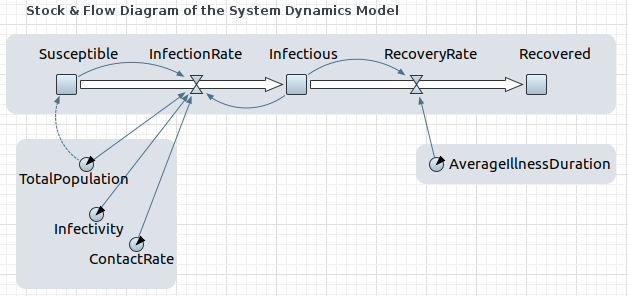
\includegraphics[width=.5\textwidth, angle=0]{./fig/SIR_SD_STOCKFLOW_DIAGRAMM.png}
	\caption{Visual System Dynamics Diagram of the SIR model in AnyLogic Personal Learning Edition 8.3.1.}
	\label{fig:sir_stockflow_diagram}
\end{figure}

Still, implementing System Dynamics directly in code is not as straight forward and involves numerical integration which can be quite tricky to get right. Thus, the aim of this paper is to look into how System Dynamics models can be implemented in code correctly without the use of a simulation package. We use the well known SIR model \cite{kermack_contribution_1927} from epidemiology to demonstrate our approach.

Our language of choice is Haskell because it emphasises a declarative programming style in which one describes \textit{what} instead of \textit{how} to compute. Further it allows to rule out interference with non-deterministic influences or side-effects already at compile-time. This is of fundamental importance for System Dynamics because it behaves completely deterministic and involves no stochastics or non-determinism whatsoever. Also, we make use of Functional Reactive Programming which allows to express continuous-time systems in a functional way. 

We show that by this approach we can arrive at correct-by-construction implementations of System Dynamic models. This means that the correctness of the code is obvious because we have closed the gap between the model specification and its implementation. Thus, the contribution of the paper is the demonstration of how to implement correct-by-construction System Dynamics simulations using Haskell and Functional Reactive Programming.

\section{Related Research}
Already noted in the Introduction, \cite{huberman_evolutionary_1993} where the first to discuss the differences update-strategies can make and introduced the terms of synchronous and asynchronous updates. They define to be synchronous as agents being updated in unison and asynchronous where one agent is updated and the others are held constant.

\medskip

\cite{a_framework_2008} give an approach for ABS on GPUs which is a very different approach to updating and iterating agents in ABS. They discuss execution order at length, highlight the problem of inducing a specific execution-order in a model which is problematic for parallel execution and give solutions how to circumvent these shortcomings. Although we haven't mapped our ideas to GPUs we explicitly include an approach for data-parallelism which, we hypothesize, can be utilized to roughly map their approach onto our terminology. 
	
\medskip
	
\cite{botta_time_2010} sketch a minimal ABS implementation in Haskell which is very similar in the basic structure of ours. This proves that our approach seems to be a very natural one to apply to Haskell. Their focus is primarily on economic simulations and instead of iterating a simulation with a global time, their focus is on how to synchronize agents which have internal, local transition times. Although their work uses Haskell as well, our focus is very different from theirs and approaches ABS in a more general and comprehensive way.

\medskip

\cite{dawson_opening_2014} describe basic inner workings of ABS environments and compare their implementation in C++ to the existing ABS environment AnyLogic which is programmed in Java. They explicitly mention asynchronous and synchronous time-models and compare them in theory but unfortunately couldn't report the results of asynchronous updates due to limited space. They interpret asynchronous time-models to be the ones in which an agent acts at random time intervals and synchronous time-models where agents are updated all in same time intervals.

\medskip

\cite{yuxuan_agent-based_2016} presents in his Master-Thesis a comprehensive discussion on how to implement an ABS for state-charts in Java and also mentions synchronous and asynchronous time-models. He identifies the asynchronous time-model to be one in which updates are triggered by the exchange of messages and the synchronous ones which trigger changes immediately without the indirection of messages.

\medskip

We observe that there seems to be a variety of meanings attributed to the terminology of asynchronous and synchronous updates but the very semantic and technical details are unclear and not described very precisely. In the next section we will address this issue by presenting the basic background and propose properties for a new terminology from which we can derive common update-strategies.

\section{Implementation: General Considerations}
All implementations of ABM/S models must solve two problems:

\begin{enumerate}
\item Agent-Implementation: how can the Agent in the model-specification be implemented?
\item Simulation-Stepping: which kind of stepping is required or best suited for the given model?
\end{enumerate}

Of course both problems influence each other and cannot be considered separated from each other.

-> Java: supports global data => suitable to implement global decisions: implementing global-time, sequential iteration with global decisions
	-> Haskell: has no global data => local decisions (has support for global data through STM/IO but then looses very power?) => implementing global-time, parallel iteration with local-decisions. 
		-> Haskell STM solution => implementing concurrent version using STM? but this is very complicated in its own right but utilizing STM it will be much more easier than in java
	-> Scala: mixed, can do both => implementing local time with random iteration and local decisions
	
\subsubsection{Agent-Implementation}
This is the process of implementing the behaviour of the Agent as specified in the model. Although there are various kinds of Agent-Models like BDI but the basic principle is always the same: sense the environment, process messages, execute actions: change environment, send messages. According to \cite{wooldridge_introduction_2009} and also influenced by Actors from \cite{agha_actors:_1986} one can abstract the abilities in each step of an Agent to be the following:

\begin{enumerate}
\item Process received messages
\item Create new Agents
\item Send messages to other Agents
\item Sense (read) the environment
\item Influence (write) the environment
\end{enumerate}

The difference between communicating with the environment and other agents is that the communication with the former one is synchronized, persists and is visible immediately (at least by the agent performing the action) whereas the communication with other agents is asynchronous.

\subsubsection{Semantics of a Simulation}
When one has implemented the model of behaviour of an Agent one needs to bring the whole simulation to life by enabling the Agents to execute their behaviour in a recurring fashion. This allows an Agent to change the environment by actions and react to changes in the environment, either by other Agents or the environment itself thus resulting in a feedback-loop. There are two ways of looking and implementing such feedback-loops. 

\paragraph{Global Stepping}
In this case the simulation is iterated in global steps where in each step each Agent is updated by running its behaviour.

\begin{enumerate}
\item \textbf{Sequential} - update one Agent after another. We assume that, given the updates are done in order of the index $i 1 to n$, then Agents $a_{n>i}$ see the updated agent-state / influence on the environment of agent $a_i$. Note that if this is not the case we would end up in the parallel-case (see next) \textit{independent} whether it is in fact running in parallel or not. For breaking deterministic ordering which could result in giving an Agent an advantage (e.g. having more information towards the end of the step) one could implement a random-walk in each step but this does not fundamentally change this approach. Also if one thinks the simulation continuously, where each step is just a very small update like in Heroes \& Cowards, then the random ordering should not change anything fundamental as no agent has real information-benefit over others as there is continuous iteration thus the agent once ahead is then behind. TODO: maybe need to make more formal

\item \textbf{Parallel} - update all Agents in parallel. This case is obviously only possible if the agents cannot interfere with each other or the environment through shared state. In this case it will make no difference how we iterate over the agents, the outcome \textit{has to be} the same - it is event-ordering invariant as all events/updates happen \textit{virtually} at the \textit{same time}. Haskell is a strong proponent of this implementation-technique.

\item \textbf{Concurrent} - update all Agents concurrently. In this case the agents run in parallel but share some state which access has to be synchronized thus introducing real random event-orderings which may or may not be desirable in the given simulation model. Can be implemented in both Java and Haskell.
\end{enumerate}

\paragraph{Local Stepping}
In this case there is no global iteration over steps but all the Agents run in parallel, doing local stepping and communicate with each other either through shared state or messages. Note that this does not impose any specific ordering of the update and can thus regarded to be real random due to its concurrent nature. It is possible to simulate the global-stepping methods from above by introducing some global locking forcing the agents into lock-step. This is the approach chosen for Scala \& Actors.

\bigskip 

The following table gives an overview of the methods presented above. Real Randomness identifies methods which produce a random ordering of their events due to their implicit workings (e.g.  concurrency) as opposed to explicit implementation (e.g random-walk of agents using a random-number generator).

TODO: add SEQ with time-advance
TODO: what about then PAR with time-advance for all? this is not logical

TODO: add actors LT (which does the time-update internal instead of being distributed by the global simulation): then again we can argue that actors ST is the same as concurrency!

\begin{table}[H]
	\center
	\begin{tabular}{ c | c | c | c | c | c }
		\textbf{Name} & \textit{Time} & \textit{Order} & \textit{Decisions} & \textit{Non-Deterministic} & \textit{Type}\\
		\hhline{=|=|=|=|=|=}
	    SEQ & Global & Sequential & Global & No & Continuous \\ 
	    \hline
	    PAR & Global & Parallel & Local & No & Discrete \\ 
	    \hline
	    CONC & Global & Concurrent & Global & Yes & Continuous \\ 
	    \hline
	    Actors ST & Global & Random & Local & Yes & Continuous \\ 
	    \hline
	    Actors RT & Local & Random & Local & Yes & Continuous \\ 
	\end{tabular}
	\caption{Summary of simulation-stepping methods.}
\end{table}



note that different types of update-strategies amount to different types of simulation . all can be used in continuous but discrete is in parallel only

semantics in interface: if the simultion is discrete, use queueMsg, if it is continuous, use sendMsg

central question is: should we hide the semantics from the sgent by providing a single interface e.g. sendMsg and make the semantic explicit only when executing the simulation or should we have different interfaces for explicit semantics e.g. sendMsg and queueMsg? the point is: when we want parallel semantics where all updates happen at once we can also run them technically in parallel. i feel we should make this explicit thus providing a queueMsg which will deliver it at the end of the iteration

global, concurrent = parallel with iterative updates where the following agents see updates. but random ordering introduced due to sync and scheduling

Each of the above presented methods imposes a different kind of event-ordering and thus all will obviously result in different \textit{absolute} simulation results. The point here is that when using ABM/S to study a system one is not interested in individual runs but in replications due to randomness and whether the system shows some emergent behaviour or not. Thus one can ask the question whether the emergent behaviour of a simulation is stable under event-ordering or not. TODO: I have no clue how to show that other than by simulations, this is also a limitation of simulations: just because it does not show up in a run it does not mean that it isn't there, just that it is unlikely - also the reverse is true: just because the emergent behaviour was there in the last n runs, does not mean it is ALWAYS there. For this we need different, more formal methods. But then again, if the level of complexity is too high we cannot solve such systems in closed form and must again fall back to simulation.

\section{Implementation in Haskell}
It is important to prevent oneself to implement an object-oriented approach in Haskell because then we would loose the power of pure functional programming. Thus the main design-considerations were:

\begin{enumerate}
\item Implement all 4 approaches mentioned in General Implementation for maximum flexibility for users of the library so they can choose which semantics of the simulation they want.
\item Pure simulation to keep up the ability to reason about it. This means to avoid running in IO Monad at all costs (except for the main-loop).
\item Utilizing STM which allows very flexible handling of state and allows running.
\item Run inside Yampa/Dunai to leverage the EDSL and continuous/discrete time-implementation.
\end{enumerate}

take haskell, add yampa and dunai and implement ActorModel on top using STM => have an ABM library in Haskell, put on hackage. NO IO!

\subsection{Utilizing STM}
with stm one can determine when everything is visible: at the end of the step or after each agent update. but this applies only to parallelism! if running agents in parallel they must execute atomically, otherwise the probability for concurrent read/writes goes to 100\% also as the number of agents goes up. if no parallelism then one final atomically at the end of each step enough. but in any case: using STM leads to the effect that agents see later updates. so really 2 cases where STM is of use in haskell: global, sequential and global concurrent

how can we implement true parallelism? can we use STM somehow or do we need local mailboxes?

\subsection{Structuring the Program}
Of course the basic pure functional primitives alone do not make a well structured functional program by themselves as the usage of classes, interfaces, objects and inheritance alone does not make a well structured object-oriented program. What is needed are \textit{patterns} how to use the primitives available in pure functional programs to arrive at well structure programs. In object-orientation much work has been done in the 90s by the highly influential book \cite{gamma_design_1994} whereas in functional programming the major inventions were also done in the 90s by the invention of Monads through \cite{Moggi1989}, \cite{Wadler1990} and \cite{Wadler1995} and beginning of the 2000s by the invention of Arrows through \cite{Hughes2000}.

\subsubsection{Higher Order Functions \& Monads}
map \& fmap, foldl, applicatives
\cite{hutton_programming_2007} gives a great overview and motivation for using fmap, applicatives and Monads. TODO: explain Monads

\subsubsection{Arrows}
\cite{Hughes2004} is a great tutorial about \textit{Arrows} which are very well suited for structuring functional programs with effects.

\begin{quote}
Just like monads, arrow types are useful for the additional operations they support, over and above those that every arrow provides.
\end{quote}

The main difference between Monads and Arrows are that where monadic computations are parameterized only over their output-type, Arrows computations are parameterised both over their input- and output-type thus making Arrows more general.

\begin{quote}
In real applications an arrow often represents some kind of a process, with an input channel of type a, and an output channel of type b.
\end{quote}

In the work \cite{Hughes2004} an example for the usage for Arrows is given in the field of circuit simulation. They use previously introduced streams to advance the simulation in discrete steps to calculate values of circuits thus the implementation is a form of \textit{discrete event simulation} - which is in the direction we are heading already with ABM/S. Also the paper mentions Yampa which is introduced in the section (TODO: reference) on functional reactive programming.

\subsubsection{Functional reactive programming (FRP)}
FRP is a paradigm for programming hybrid systems which combine continuous and discrete components. Time is explicitly modelled: there is a continuous and synchronous time flow.  \\

there have been many attempts to implement FRP in frameworks which each has its own pro and contra. all started with fran, a domain specific language for graphics and animation and at yale FAL, Frob, Fvision and Fruit were developed. The ideas of them all have then culminated in Yampa which is the reason why it was chosen as the FRP framework. Also, compared to other frameworks it does not distinguish between discrete and synchronous time but leaves that to the user of the framework how the time flow should be sampled (e.g. if the sampling is discrete or continuous - of course sampling always happens at discrete times but when we speak about discrete sampling we mean that time advances in natural numbers: 1,2,3,4,... and when speaking of continuous sampling then time advances in fractions of the natural numbers where the difference between each step is a real number in the range of [0..1]) \\

time- and space-leak: when a time-dependent computation falls behind the current time. TODO: give reason why and how this is solved through Yampa. \\
Yampa solves this by not allowing signals as first-class values but only allowing signal functions which are signal transformers which can be viewed as a function that maps signals to signals. A signal function is of type SF which is abstract, thus it is not possible to build arbitrary signal functions. Yampa provides primitive signal functions to define more complex ones and utilizes arrows \cite{Hughes2004} to structure them where Yampa itself is built upon the arrows: SF is an instance of the Arrow class. \\

Fran, Frob and FAL made a significant distinction between continuous values and discrete signals. Yampas distinction between them is not as great. Yampas signal-functions can return an Event which makes them then to a signal-stream - the event is then similar to the Maybe type of Haskell: if the event does not signal then it is NoEvent but if it Signals it is Event with the given data. Thus the signal function always outputs something and thus care must be taken that the frequency of events should not exceed the sampling rate of the system (sampling the continuous time-flow). TODO: why? what happens if events occur more often than the sampling interval? will they disappear or will the show up every time? \\

switches allow to change behaviour of signal functions when an event occurs. there are multiple types of switches: immediate or delayed, once-only and recurring - all of them can be combined thus making 4 types. It is important to note that time starts with 0 and does not continue the global time when a switch occurs. TODO: why was this decided? \\

\cite{Nilsson2002} give a good overview of Yampa and FRP. Quote: "The essential abstraction that our system captures is time flow". Two \textit{semantic} domains for progress of time: continuous and discrete. \\

The first implementations of FRP (Fran) implemented FRP with synchronized stream processors which was also followed by \cite{Wan2000}. Yampa is but using continuations inspired by Fudgets. In the stream processors approach "signals are represented as time-stamped streams, and signal functions are just functions from streams to streams", where "the Stream type can be implemented directly as (lazy) list in Haskell...":
\begin{lstlisting}[frame=single]
type Time = Double
type SP a b = Stream a -> Stream b
newtype SF a b = SF (SP (Time, a) b)
\end{lstlisting}
Continuations on the other hand allow to freeze program-state e.g. through closures and partial applications in functions which can be continued later. This requires an indirection in the Signal-Functions which is introduced in Yampa in the following manner. 
\begin{lstlisting}[frame=single]
type DTime = Double

data SF a b = 
	SF { sfTF :: DTime -> a -> (SF a b, b)
\end{lstlisting}
The implementer of Yampa call a signal function in this implementation a \textit{transition function}. It takes the amount of time which has passed since the previous time step and the durrent input signal (a). It returns a \textit{continuation} of type SF a b determining the behaviour of the signal function on the next step (note that exactly this is the place where how one can introduce stateful functions like integral: one just returns a new function which encloses inputs from the previous time-step) and an \textit{output sample} of the current time-step. \\

When visualizing a simulation one has in fact two flows of time: the one of the user-interface which always follows real-time flow, and the one of the simulation which could be sped up or slowed down. Thus it is important to note that if I/O of the user-interface (rendering, user-input) occurs within the simulations time-frame then the user-interfaces real-time flow becomes the limiting factor. Yampa provides the function embedSync which allows to embed a signal function within another one which is then run at a given ratio of the outer SF. This allows to give the simulation its own time-flow which is independent of the user-interface. \\

One may be initially want to reject Yampa as being suitable for ABM/S because one is tempted to believe that due to its focus on continuous, time-changing signals, Yampa is only suitable for physical simulations modelled explicitly using mathematical formulas (integrals, differential equations,...) but that is not the case. Yampa has been used in multiple agent-based applications: \cite{Hudak2003} uses Yampa for implementing a robot-simulation, \cite{Courtney2003} implement the classical Space Invaders game using Yampa, the thesis of \cite{Meisinger2010} shows how Yampa can be used for implementing a Game-Engine, \cite{Frag2005} implemented a 3D first-person shooter game with the style of Quake 3 in Yampa. Note that although all these applications don't focus explicitly on agents and agent-based modelling / simulation all of them inherently deal with kinds of agents which share properties of classical agents: game-entities, robots,... Other fields in which Yampa was successfully used were programming of synthesizers (TODO: cite), Network Routers, Computer Music Development and various other computer-games. This leads to the conclusion that Yampa is mature, stable and suitable to be used in functional ABM/S. \\
Jason Gregory (Game Engine Architecture) defines Computer-Games as "soft real-time interactive agent-based computer simulations".

To conclude: when programming systems in Haskell and Yampa one describes the system in terms of signal functions in a declarative manner (functional programming) using the EDSL of Yampa. During execution the top level signal functions will then be evaluated and return new signal functions (transition functions) which act as continuations: "every signal function in the dataflow graph returns a new continuation at every time step".

"A major design goal for FRP is to free the programmer from 'presentation' details by providing the ability to think in terms of 'modeling'. It is common that an FRP program is concise enough to also serve as a specification for the problem it solves" \cite{Wan2000}. This quotation describes exactly one of the strengths using FRP in ACE \\

\subsubsection{Dunai}
TODO: \cite{perez_functional_2016}

\subsection{Putting it all together}

\section{Prototyping}

\graphicspath{{./fig/}}	%specifying the folder for the figures

The coordinates calculated by the agents are \textit{virtual} ones ranging between 0.0 and 1.0. This prevents us from knowing the rendering-resolution and polluting code which has nothing to do with rendering with these implementation-details. Also this simulation could run without rendering-output or any rendering-frontend thus sticking to virtual coordinates is also very useful regarding this (but then again: what is the use of this simulation without any visual output=


\subsection{Reasoning}
Allowing to reason about a program is one of the most interesting and powerful features of a Haskell-program. Just by looking at the types one can show that there is no randomness in the simulation \textit{after} the random initialization, which is not slightest possible in the case of a Java, Scala, ReLogo or NetLogo solution. Things we can reason about just by looking at types:

\begin{itemize}
\item Concurrency involved?
\item Randomness involved?
\item IO with the system (e.g. user-input, read/write to file(s),...) involved?
\item Termination?
\end{itemize}

This all boils down to the question of whether there are \textit{side-effects} included in the simulation or not.

What about reasoning about the termination? Is this possible in Haskell? Is it possible by types alone? My hypothesis is that the types are an important hint but are not able to give a clear hint about termination and thus we we need a closer look at the implementation. In dependently-typed programming languages like Agda this should be then possible and the program is then also a 
proof that the program itself terminates.

reasoning about Heros \& Cowards: what can we deduce from the types? what can we deduce from the implementation?\\

Compare the pure-version (both Yampa and classic) with the IO-version of haskell: we loose basically all power to reason by just looking at the types as all kind of side-effects are possible when running in the IO-Monad.

in haskell pure version i can guarantee by reasoning and looking at the types that the update strategy will be simultaneous deterministic. i cant do that in java

TODO: implement haskell-version with shared-state (STM primitives) without using IO
TODO: implement haskell-version which defines abstract types for the simulation


\subsubsection{The type of a Simulation}
the type of a simulation: try to define the most general types of a simulation and then do reasoning about it

simulation :: Model -> Double -> Int -> [Model]

step :: Model -> Double -> Model

TODO: can we say something about the methods Model can/must/should support?

\subsection{Debugging \& Testing}
Because functions compose easier than classes \& objects (TODO: we need hard claims here, look for literature supporting this thesis or proof it by myself) it is also much easier to debug \textit{parts} of the implementation e.g. the rendering of the agents without any changes to the system as a whole - just the main-loop has do be adopted. Then it is very easy to calculate e.g. only one iteration and to freeze the result or to manually create agents instead of randomly create initial ones.

TODO: quickcheck \cite{claessen_quickcheck:_2000}


\subsection{Lazy Evaluation}
can specify to run the simulation for an unlimited number of steps but only the ones which are required so far are calculated.

\subsection{Performance}
Java outperforms Haskell implementation easily with 100.000 Agents - at first not surprising because of in-place updates of friend and enemies and no massive copy-overhead as in haskell. But look WHERE exactly we loose / where the hotspots are in both solutions. 1000.000 seems to be too much even for the Java-implementation.

\subsection{Numerical Stability}
The agents in the Java-implementation collapsed after a given number of iterations into a single point as during normalization of the direction-vector the length was calculated to be 0. This could be possible if agents come close enough to each other e.g. in the border-worldtype it was highly probable after some iterations when enough agents have assembled at the borders whereas in the Wrapping-WorldType it didn't occur in any run done so far. \\
In the case of a 0-length vector a division by 0  resulting in NaN which \textit{spread} through the network of neighbourhood as every agent calculated its new position it got \textit{infected} by the NaN of a neighbour at some point. The solution was to simply return a 0-vector instead of the normalized which resulted in no movement at all for the current iteration step of the agent. 


\subsection{Update-Strategies}
\begin{enumerate}
\item All states are copied/frozen which has the effect that all agents update their positions \textit{simultaneously}
\item Updating one agent after another utilizing aliasing (sharing of references) to allow agents updated \textit{after} agents before to see the agents updated before them. Here we have also two strategies: deterministic- and random-traversal.
\item Local observations: Akka
\end{enumerate}

\subsection{Different results with different Update-Strategies?}
Problem: the following properties have to be the same to reproduce the same results in different implementations: \\

Same initial data: Random-Number-Generators
Same numerical-computation: floating-point arithmetic
Same ordering of events: update-strategy, traversal, parallelism, concurrency

\begin{itemize}
\item Same Random-Number Generator (RNG) algorithm which must produce the same sequence given the same initial seed.
\item Same Floating-Point arithmetic
\item Same ordering of events: in Scala \& Actors this is impossible to achieve because actors run in parallel thus relying on os-specific non-deterministic scheduling. Note that although the scheduling algorithm is of course deterministic in all os (i guess) the time when a thread is scheduled depends on the current state of the system which can change all the time due to \textit{very} high number of variables outside of influence (some of the non-deterministic): user-input, network-input, .... which in effect make the system appear as non-deterministic due to highly complex dependencies and feedback.
\item Same dt sequence => dt MUST NOT come from GUI/rendering-loop because gui/rendering is, as all parallelism/concurency subject to performance variations depending on scheduling and load of OS.
\end{itemize}

It is possible to compare the influences of update-strategies in the Java implementation by running two exact simulations (agentcount, speed, dt, herodistribution, random-seed, world-type) in lock-step and comparing the positions of the agent-pairs with same ids after each iteration. If either the x or y coordinate is no equal then the positions are defined to be \textit{not} equal and thus we assume the simulations have then diverged from each other. \\
It is clear that we cannot compare two floating-point numbers by trivial == operator as floating-point numbers always suffer rounding errors thus introducing imprecision. What may seem to be a straight-forward solution would be to introduce some epsilon, measuring the absolute error: abs(x1 - x2) > epsilon, but this still has its pitfalls. The problem with this is that, when number being compared are very small as well then epsilon could be far too big thus returning to be true despite the small numbers are compared to each other quite different. Also if the numbers are very large the epsilon could end up being smaller than the smallest rounding error, so that this comparison will always return false. The solution would be to look at the \textit{relative error}: abs((a-b)/b) < epsilon. \\
The problem of introducing a relative error is that in our case although the relative error can be very small the comparison could be determined to be different but looking in fact exactly the same without being able to be distinguished with the eye. Thus we make use of the fact that our coordinates are virtual ones, always being in the range of [0..1] and are falling back to the measure of absolute error with an epsilon of 0.1. Why this big epsilon? Because this will then definitely show us that the simulation is \textit{different}. \\

The question is then which update-strategies lead to diverging results. The hypothesis is that when doing simultaneous updates it should make no difference when doing random-traversal or deterministic traversal => when comparing two simulations with simultaneous updates and all the same except first random- and the other deterministic traversal then they should never diverge. Why? Because in the simultaneous updates there is no ordering introduce, all states are frozen and thus the ordering of the updates should have no influence, \textit{both simulations should never diverge, \textbf{independent how dt and epsilon are selected}}. \\
Do the simulation-results support the hypothesis? Yes they support the hypothesis - even in the worst cast with very large dt compared to epsilon (e.g. dt = 1.0, epsilon = 1.0-12)

The 2nd hypothesis is then of course that when doing consecutive updates the simulations will \textit{always} diverge independent when having different traversal-strategies. \\
Simulations show that the selection of \textit{dt} is crucial in how fast the simulations diverge when using different traversal-strategies. The observation is that \textit{The larger dt the faster they diverge and the more substantial and earlier the divergence.}. Of course it is not possible to proof using simulations alone that they will always diverge when having different traversal-strategies. Maybe looking at the dynamics of the error (the maximum of the difference of the x and y pairs) would reveal some insight? \\

The 3rd hypothesis is that the number of agents should also lead to increased speed of divergence when having different traversal-strategies. This could be shown when going from 60 agents with a dt of 0.01 which never exceeded a global error of 0.02 to 6000 agents which after 3239 steps exceeded the absolute error of 0.1.

\subsection{Reproducing Results in different Implementations}
actors: time is always local and thus information as well. if we fall back to a global time like system time we would also fall back to real-time. anyway in distributed systems clock sync is a very non-trivial problem and inherently not possible (really?). thus using some global clock on a metalevel above/outside the simulation will only buy us more problems than it would solve us. real-time does not help either as it is never hard real time and thus also unpredictable: if one tells the actor to send itself a message after 100ms then one relies on the capability of the OS-timer and scheduler to schedule exactly after 100ms: something which is always possible thus 100ms are never hard 100ms but soft with variations.

qualitative comparison: print pucture with patterns. all implementations are able to reproduce these patterns independent from the update strategy

no need to compare individual runs and waste time in implementing RNGs, what is more interesting is whether the qualitative results are the same: does the system show the same emergent behaviour? Of course if we can show that the system will behave exactly the same then it will also exhibit the same emergent behaviour but that is not possible under some circumstances e.g. the simulation-runs of Akka are always unique and never comparable due to random event-ordering produced by concurrency \& scheduling. Also we don't have to proof the obvious: given the same algorithm, the same random-data, the same treatment of numbers and the same ordering of events, the outcome \textit{must} be the same, otherwise there are bugs in the program. Thus when comparing results given all the above mentioned properties are the same one in effect tests only if the programs contain no bugs - or the same bugs, if they \textit{are the same}. \\

Thus we can say: the systems behave qualitatively the same under different event-orderings.

Thus the essence of this boils down to the question: "Is the emergent behaviour of the system is stable under random/different/varying event-ordering?". In this case it seems to be so as proofed by the Akka implementation. In fact this is a very desirable property of a system showing emergent behaviour but we need to get much more precise here: what is an event? what is an emergent behaviour of a system? what is random-ordering of events? (Note: obviously we are speaking about repeated runs of a system where the initial conditions may be the same but due to implementation details like concurrency we get a different event-ordering in each simulation-run, thus the event-orderings vary between runs, they can be in fact be regarded as random).

\begin{figure}[H]
	\centering
  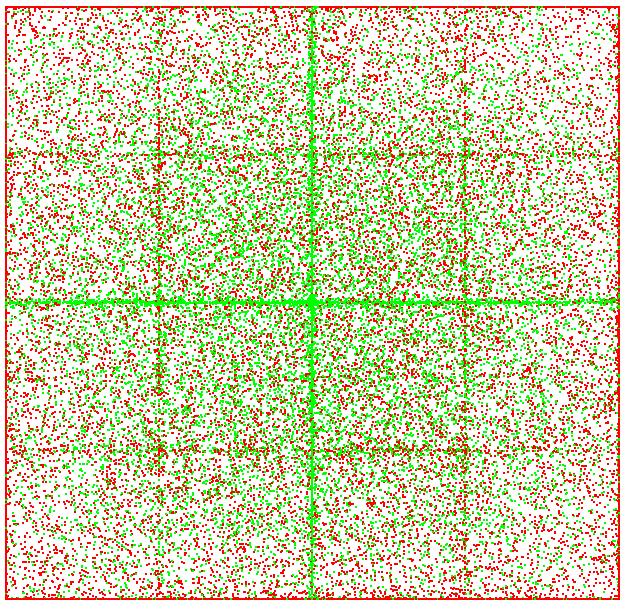
\includegraphics[width=1.0\textwidth, angle=0]{EMERGENT_PATTERN.png}
  	\caption{The emergent pattern used as criteria for qualitative comparison of implementations. Note the big green cross in the center and the smaller red crosses in each sub-sector. World-type is \textit{border} with 100.000 Agents where 25\% are Heroes.}
	\label{fig:EMERGENT_PATTERN}
\end{figure}


\subsection{Problem of RNG}
Have to behave EXACTLY The same: VERY difficult because of differing interfaces e.g. compare java to haskell RNGs.
Solution: create a deterministic RNG generating a number-stream starting from 1 and just counting up. The program should work also in this case, if not, something should be flawed!

Peer told me to implement a RNG-Trace: generate a list of 1000.0000 pre-calculated random-numbers in range of [0..1], store them in a file and read the trace in all implementations. Needs lots of implementation.

\subsection{Run-Time Complexity}
what if the number of agents grows? how does the run-time complexity of the simulation increases? Does it differ from implementation to implementation? The model is O(n) but is this true for the implementation?

\subsection{Simulation-Loops}
There are at least 2 parts to implementing a simulation: 1. implementing the logic of an agent and 2. implementing the iteration/recursion which drives the whole simulation

Classic \\
Yampa \\ TODO: use par to parallelize
Gloss \\
gloss provides means for simple simulation using simulate method. But: are all ABM systems like that?

\subsection{Agent-Representation}
Java: (immutable) Object
Haskell Classic: a struct
Haskell Yampa: a Signal-Function
Gloss: same as haskell classic
Akka: Actors

\subsection{EDSL}
simplify simulation into concise EDSL: distinguish between different kind if sims: continuous/discrete iteration on: fixed set, growing set, shrinking set, dynamic set. 

\section{Results}

\graphicspath{{./fig/}}	%specifying the folder for the figures

The coordinates calculated by the agents are \textit{virtual} ones ranging between 0.0 and 1.0. This prevents us from knowing the rendering-resolution and polluting code which has nothing to do with rendering with these implementation-details. Also this simulation could run without rendering-output or any rendering-frontend thus sticking to virtual coordinates is also very useful regarding this (but then again: what is the use of this simulation without any visual output=


\subsection{Reasoning}
Allowing to reason about a program is one of the most interesting and powerful features of a Haskell-program. Just by looking at the types one can show that there is no randomness in the simulation \textit{after} the random initialization, which is not slightest possible in the case of a Java, Scala, ReLogo or NetLogo solution. Things we can reason about just by looking at types:

\begin{itemize}
\item Concurrency involved?
\item Randomness involved?
\item IO with the system (e.g. user-input, read/write to file(s),...) involved?
\item Termination?
\end{itemize}

This all boils down to the question of whether there are \textit{side-effects} included in the simulation or not.

What about reasoning about the termination? Is this possible in Haskell? Is it possible by types alone? My hypothesis is that the types are an important hint but are not able to give a clear hint about termination and thus we we need a closer look at the implementation. In dependently-typed programming languages like Agda this should be then possible and the program is then also a 
proof that the program itself terminates.

reasoning about Heros \& Cowards: what can we deduce from the types? what can we deduce from the implementation?\\

Compare the pure-version (both Yampa and classic) with the IO-version of haskell: we loose basically all power to reason by just looking at the types as all kind of side-effects are possible when running in the IO-Monad.

in haskell pure version i can guarantee by reasoning and looking at the types that the update strategy will be simultaneous deterministic. i cant do that in java

TODO: implement haskell-version with shared-state (STM primitives) without using IO
TODO: implement haskell-version which defines abstract types for the simulation


\subsubsection{The type of a Simulation}
the type of a simulation: try to define the most general types of a simulation and then do reasoning about it

simulation :: Model -> Double -> Int -> [Model]

step :: Model -> Double -> Model

TODO: can we say something about the methods Model can/must/should support?

\subsection{Debugging \& Testing}
Because functions compose easier than classes \& objects (TODO: we need hard claims here, look for literature supporting this thesis or proof it by myself) it is also much easier to debug \textit{parts} of the implementation e.g. the rendering of the agents without any changes to the system as a whole - just the main-loop has do be adopted. Then it is very easy to calculate e.g. only one iteration and to freeze the result or to manually create agents instead of randomly create initial ones.

TODO: quickcheck \cite{claessen_quickcheck:_2000}


\subsection{Lazy Evaluation}
can specify to run the simulation for an unlimited number of steps but only the ones which are required so far are calculated.

\subsection{Performance}
Java outperforms Haskell implementation easily with 100.000 Agents - at first not surprising because of in-place updates of friend and enemies and no massive copy-overhead as in haskell. But look WHERE exactly we loose / where the hotspots are in both solutions. 1000.000 seems to be too much even for the Java-implementation.

\subsection{Numerical Stability}
The agents in the Java-implementation collapsed after a given number of iterations into a single point as during normalization of the direction-vector the length was calculated to be 0. This could be possible if agents come close enough to each other e.g. in the border-worldtype it was highly probable after some iterations when enough agents have assembled at the borders whereas in the Wrapping-WorldType it didn't occur in any run done so far. \\
In the case of a 0-length vector a division by 0  resulting in NaN which \textit{spread} through the network of neighbourhood as every agent calculated its new position it got \textit{infected} by the NaN of a neighbour at some point. The solution was to simply return a 0-vector instead of the normalized which resulted in no movement at all for the current iteration step of the agent. 


\subsection{Update-Strategies}
\begin{enumerate}
\item All states are copied/frozen which has the effect that all agents update their positions \textit{simultaneously}
\item Updating one agent after another utilizing aliasing (sharing of references) to allow agents updated \textit{after} agents before to see the agents updated before them. Here we have also two strategies: deterministic- and random-traversal.
\item Local observations: Akka
\end{enumerate}

\subsection{Different results with different Update-Strategies?}
Problem: the following properties have to be the same to reproduce the same results in different implementations: \\

Same initial data: Random-Number-Generators
Same numerical-computation: floating-point arithmetic
Same ordering of events: update-strategy, traversal, parallelism, concurrency

\begin{itemize}
\item Same Random-Number Generator (RNG) algorithm which must produce the same sequence given the same initial seed.
\item Same Floating-Point arithmetic
\item Same ordering of events: in Scala \& Actors this is impossible to achieve because actors run in parallel thus relying on os-specific non-deterministic scheduling. Note that although the scheduling algorithm is of course deterministic in all os (i guess) the time when a thread is scheduled depends on the current state of the system which can change all the time due to \textit{very} high number of variables outside of influence (some of the non-deterministic): user-input, network-input, .... which in effect make the system appear as non-deterministic due to highly complex dependencies and feedback.
\item Same dt sequence => dt MUST NOT come from GUI/rendering-loop because gui/rendering is, as all parallelism/concurency subject to performance variations depending on scheduling and load of OS.
\end{itemize}

It is possible to compare the influences of update-strategies in the Java implementation by running two exact simulations (agentcount, speed, dt, herodistribution, random-seed, world-type) in lock-step and comparing the positions of the agent-pairs with same ids after each iteration. If either the x or y coordinate is no equal then the positions are defined to be \textit{not} equal and thus we assume the simulations have then diverged from each other. \\
It is clear that we cannot compare two floating-point numbers by trivial == operator as floating-point numbers always suffer rounding errors thus introducing imprecision. What may seem to be a straight-forward solution would be to introduce some epsilon, measuring the absolute error: abs(x1 - x2) > epsilon, but this still has its pitfalls. The problem with this is that, when number being compared are very small as well then epsilon could be far too big thus returning to be true despite the small numbers are compared to each other quite different. Also if the numbers are very large the epsilon could end up being smaller than the smallest rounding error, so that this comparison will always return false. The solution would be to look at the \textit{relative error}: abs((a-b)/b) < epsilon. \\
The problem of introducing a relative error is that in our case although the relative error can be very small the comparison could be determined to be different but looking in fact exactly the same without being able to be distinguished with the eye. Thus we make use of the fact that our coordinates are virtual ones, always being in the range of [0..1] and are falling back to the measure of absolute error with an epsilon of 0.1. Why this big epsilon? Because this will then definitely show us that the simulation is \textit{different}. \\

The question is then which update-strategies lead to diverging results. The hypothesis is that when doing simultaneous updates it should make no difference when doing random-traversal or deterministic traversal => when comparing two simulations with simultaneous updates and all the same except first random- and the other deterministic traversal then they should never diverge. Why? Because in the simultaneous updates there is no ordering introduce, all states are frozen and thus the ordering of the updates should have no influence, \textit{both simulations should never diverge, \textbf{independent how dt and epsilon are selected}}. \\
Do the simulation-results support the hypothesis? Yes they support the hypothesis - even in the worst cast with very large dt compared to epsilon (e.g. dt = 1.0, epsilon = 1.0-12)

The 2nd hypothesis is then of course that when doing consecutive updates the simulations will \textit{always} diverge independent when having different traversal-strategies. \\
Simulations show that the selection of \textit{dt} is crucial in how fast the simulations diverge when using different traversal-strategies. The observation is that \textit{The larger dt the faster they diverge and the more substantial and earlier the divergence.}. Of course it is not possible to proof using simulations alone that they will always diverge when having different traversal-strategies. Maybe looking at the dynamics of the error (the maximum of the difference of the x and y pairs) would reveal some insight? \\

The 3rd hypothesis is that the number of agents should also lead to increased speed of divergence when having different traversal-strategies. This could be shown when going from 60 agents with a dt of 0.01 which never exceeded a global error of 0.02 to 6000 agents which after 3239 steps exceeded the absolute error of 0.1.

\subsection{Reproducing Results in different Implementations}
actors: time is always local and thus information as well. if we fall back to a global time like system time we would also fall back to real-time. anyway in distributed systems clock sync is a very non-trivial problem and inherently not possible (really?). thus using some global clock on a metalevel above/outside the simulation will only buy us more problems than it would solve us. real-time does not help either as it is never hard real time and thus also unpredictable: if one tells the actor to send itself a message after 100ms then one relies on the capability of the OS-timer and scheduler to schedule exactly after 100ms: something which is always possible thus 100ms are never hard 100ms but soft with variations.

qualitative comparison: print pucture with patterns. all implementations are able to reproduce these patterns independent from the update strategy

no need to compare individual runs and waste time in implementing RNGs, what is more interesting is whether the qualitative results are the same: does the system show the same emergent behaviour? Of course if we can show that the system will behave exactly the same then it will also exhibit the same emergent behaviour but that is not possible under some circumstances e.g. the simulation-runs of Akka are always unique and never comparable due to random event-ordering produced by concurrency \& scheduling. Also we don't have to proof the obvious: given the same algorithm, the same random-data, the same treatment of numbers and the same ordering of events, the outcome \textit{must} be the same, otherwise there are bugs in the program. Thus when comparing results given all the above mentioned properties are the same one in effect tests only if the programs contain no bugs - or the same bugs, if they \textit{are the same}. \\

Thus we can say: the systems behave qualitatively the same under different event-orderings.

Thus the essence of this boils down to the question: "Is the emergent behaviour of the system is stable under random/different/varying event-ordering?". In this case it seems to be so as proofed by the Akka implementation. In fact this is a very desirable property of a system showing emergent behaviour but we need to get much more precise here: what is an event? what is an emergent behaviour of a system? what is random-ordering of events? (Note: obviously we are speaking about repeated runs of a system where the initial conditions may be the same but due to implementation details like concurrency we get a different event-ordering in each simulation-run, thus the event-orderings vary between runs, they can be in fact be regarded as random).

\begin{figure}[H]
	\centering
  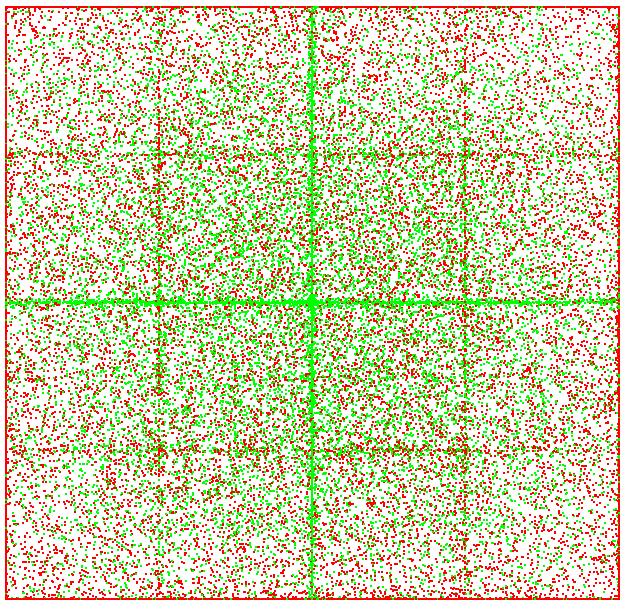
\includegraphics[width=1.0\textwidth, angle=0]{EMERGENT_PATTERN.png}
  	\caption{The emergent pattern used as criteria for qualitative comparison of implementations. Note the big green cross in the center and the smaller red crosses in each sub-sector. World-type is \textit{border} with 100.000 Agents where 25\% are Heroes.}
	\label{fig:EMERGENT_PATTERN}
\end{figure}


\subsection{Problem of RNG}
Have to behave EXACTLY The same: VERY difficult because of differing interfaces e.g. compare java to haskell RNGs.
Solution: create a deterministic RNG generating a number-stream starting from 1 and just counting up. The program should work also in this case, if not, something should be flawed!

Peer told me to implement a RNG-Trace: generate a list of 1000.0000 pre-calculated random-numbers in range of [0..1], store them in a file and read the trace in all implementations. Needs lots of implementation.

\subsection{Run-Time Complexity}
what if the number of agents grows? how does the run-time complexity of the simulation increases? Does it differ from implementation to implementation? The model is O(n) but is this true for the implementation?

\subsection{Simulation-Loops}
There are at least 2 parts to implementing a simulation: 1. implementing the logic of an agent and 2. implementing the iteration/recursion which drives the whole simulation

Classic \\
Yampa \\ TODO: use par to parallelize
Gloss \\
gloss provides means for simple simulation using simulate method. But: are all ABM systems like that?

\subsection{Agent-Representation}
Java: (immutable) Object
Haskell Classic: a struct
Haskell Yampa: a Signal-Function
Gloss: same as haskell classic
Akka: Actors

\subsection{EDSL}
simplify simulation into concise EDSL: distinguish between different kind if sims: continuous/discrete iteration on: fixed set, growing set, shrinking set, dynamic set. 

\section{Conclusion and further research}

So far we only looked at recursive simulation in a simulation with a strictly sequential update-strategy where agents are updated in sequence after each other as defined in TODO: cite my Art-Of-Iteration Paper. We leave the question of how Meta-ABS would apply to the parallel update-strategy and whether it is reasonable to extend it to that strategy or not for further research.

Research Questions
\begin{enumerate}
	\item How does deep regression influence the dynamics of a system? Hypothesis: TODO
	\item How do the dynamics of a system change when using perfect information or learning local information? Hypothesis: TODO
	\item Is a hidden markov model suitable for the local learning? Hypothesis: TODO
	\item How can MetaABS best be implemented? Hypothesis: implementing a MetaABS EDSL in a pure functional language like Haskell, should be best suited due to its inherent recursive, declarative nature, which should allow a direct mapping of features of this paradigm to the specification of the meta-model
\end{enumerate}

Problems
\begin{itemize}
	\item Definition of a recursive, declarative description of the Model.
	\item Perfect information about other agents is not realistic and runs counter to agent-based simulation (especially in social sciences) thus an Agent needs to be able to have local, noisy representations of the other agents.
	\item Local representation of other agents could be captured by Hidden Markov Models: observe what other agents do but have hidden interpretation of their internal state - these internal state-representations can be different between the local and the global version whereas the agent learns to represent the global version as best as possible locally.
	\item Infinite regress is theoretically possible but not on computers, we need to terminate at some point
\end{itemize}

\section{Further Research}

\subsection{Multi-Step Conversations}
The communication in this simulation is single-step unidirectional: in each step of the simulation an agent looks at the position of the enemy and friend and updates its position, there is no conversation going on between the agent and its friend and enemy thus making it single-step and unidirectional because the whole information flow is initiated from one agent and no response is given. This is becomes kind of relaxed in the Scala implementation but is still basically unidirectional and single-step - the agents don't engage in a conversation. In many ABM/S models this is perfectly reasonable because many of the models work this way but when having e.g. bartering processes like in agent-based computational economics (ACE) where agents have a conversation with multiple asks and bids to find a price they are happy with, this method becomes obviously too restricted. \\ The author investigates exactly this problem in an additional paper, where he looks at how to implement bartering-processes in ACE using Akka and Haskell (bidirectional multi-step conversations)

\subsection{LISP}
LISP is the oldest functional programming language and the second-oldest high-level programming language, only one year younger than Fortran. It would have been very interesting to research how we can do ABM/S in LISP utilizing its \textit{homoiconicity} but that would have opened up too much complexity also because LISP, despite being a functional programming language, is too far away from both Haskell and Scala. Thus the topic of applying LISP to ABM/S is left for further research in another paper. 

\subsection{Process-Calculi}
There is a strong connection of the ideas between the Actor-Model and Process-Calculi like the Pi-Calculus (TODO: cite Milner) and research has been done on connecting both worlds (TODO: cite Agha Gul). Also because the Actor-Model is so close to Agents because it was a major inspiration for the development of Agents and thus be regarded as one way of implementing Agents, one can argue due to transitivity that Agents can be connected to Pi-Calculus as well. This would allow to formalize Agents using the algebraic power and tools developed in Pi-Calculus.

\newpage

\bibliographystyle{acm}
\bibliography{../../references/phdReferences.bib}


\end{document}